\documentclass[conference]{IEEEtran}
\IEEEoverridecommandlockouts
\usepackage{cite}
\usepackage{amsmath,amssymb,amsfonts}
\usepackage{algorithmic}
\usepackage{graphicx}
\usepackage{textcomp}
\usepackage{xcolor}
\usepackage{booktabs}
\usepackage{float}
\usepackage[hidelinks]{hyperref}

\begin{document}

\title{When Geometry Misleads: Evaluating Semantic Fidelity in Latent Transition Models for LLM Reasoning\\

}

\author{\IEEEauthorblockN{Vaibhav Singh}
\IEEEauthorblockA{Email: singhvaibhavip@gmail.com \\
}
}

\maketitle

\begin{abstract}
Latent reasoning seeks to perform intermediate computation directly in the hidden-state space of a language model, potentially reducing the need for repeated autoregressive decoding. However, evaluating whether a predicted latent state represents the \textit{correct next reasoning state} remains challenging. Standard geometric objectives such as cosine similarity or mean-squared error measure proximity in representation space, but proximity alone does not establish semantic correctness.

We introduce \textbf{LatentBench}, a framework for evaluating semantic fidelity in latent transition models using a frozen language-model teacher, task-level representation probes, oracle transitions, and action-control ablations. The framework separates geometric reconstruction from semantic state advancement through \textbf{Semantic Gain} and \textbf{Oracle Gap}, while simultaneously tracking cosine similarity, mean-centered cosine similarity, mean-squared error, and probe accuracy.

We evaluate Linear, MLP, and Transformer transition models on the Countdown task using a frozen TinyLlama teacher, with three independent seeds per architecture. Across the nine audited experimental conditions, all three architectures exhibit consistently non-zero Oracle Gaps while maintaining high raw cosine similarity. Mean Oracle Gap is 0.1944 for Linear, 0.1788 for MLP, and 0.1860 for Transformer. All nine audited runs produced negative True Action Semantic Gain, indicating limited semantic advancement despite strong geometric proximity to the current representation.

A Welch's ANOVA does not detect a statistically significant architecture effect on Oracle Gap ($F(2,3.59)=1.1748, p=0.4050$). Pairwise Welch tests with Holm correction likewise do not reach statistical significance. Because only three seeds are available per architecture, these results should be interpreted as \textbf{inconclusive with respect to fine-grained architectural differences rather than as evidence of equivalence}.

Our results demonstrate that, in the evaluated Countdown and TinyLlama setting, geometric similarity alone can substantially overstate the semantic fidelity of latent transitions. The findings motivate evaluation protocols that explicitly measure task-relevant semantic state preservation rather than relying solely on representation-level reconstruction metrics.
\end{abstract}

\begin{IEEEkeywords}
Latent Reasoning, Representation Learning, World Models, Mechanistic Interpretability, Joint-Embedding Predictive Architecture (JEPA), Linear Probing
\end{IEEEkeywords}

\section{Introduction}

Large language models perform reasoning through a sequence of internal computations that ultimately produce an autoregressive sequence of tokens. An appealing alternative is to perform some of this computation directly in the model's latent representation space. Instead of repeatedly invoking the full language model to generate intermediate reasoning states, a learned transition model could attempt to advance a hidden representation from one reasoning state to the next. Such latent transitions could potentially provide a more compact mechanism for multi-step computation while avoiding explicit token-level intermediate generation.

This approach raises a fundamental evaluation question: \textbf{when a transition model predicts a new latent state, how can we determine whether that state actually represents the correct next step of reasoning?} A predicted representation may be numerically close to its input while failing to encode the semantic change required by the task. Consequently, evaluating latent transitions exclusively through geometric reconstruction metrics such as cosine similarity or mean-squared error may provide an incomplete picture of their actual reasoning behavior.

This distinction becomes particularly important in high-dimensional language-model representation spaces. Representations can exhibit substantial local similarity even when their task-relevant content differs. A transition model that changes the latent state only minimally may therefore obtain a high cosine similarity score without successfully advancing the underlying reasoning process. Conversely, a semantically meaningful transition need not necessarily correspond to the largest possible geometric displacement. An evaluation methodology therefore requires a mechanism for distinguishing \textbf{representation proximity} from \textbf{semantic state preservation}.

We address this problem with \textbf{LatentBench}, an evaluation framework designed to measure semantic fidelity during latent-state transitions. Rather than treating geometric reconstruction as a sufficient objective, LatentBench introduces an oracle-based semantic reference and evaluates predicted states through task-relevant representation probes. The framework measures \textbf{Semantic Gain}, which captures semantic advancement relative to the relevant baseline, and \textbf{Oracle Gap}, which quantifies the difference between the semantic behavior of a learned transition and the corresponding oracle transition. Action-conditioned, shuffled-action, constant-action, and action-blind controls further test whether a transition model meaningfully responds to the action supplied to it. 

We use this framework to study three transition-model families---Linear, MLP, and Transformer---operating over representations produced by a frozen TinyLlama teacher on the Countdown task. The empirical study uses 5,000 training problems, 500 validation problems, and 1,000 test problems, with three independent random seeds (42, 43, and 44) for each architecture. The resulting experiments allow us to examine both the absolute semantic fidelity of latent transitions and whether increasing transition-model capacity changes their behavior.

The results reveal a consistent geometry--semantics discrepancy. Raw cosine similarity remains high across the evaluated architectures, while True Action Semantic Gain is generally negative and Oracle Gap remains substantial. Thus, although the more expressive transition models exhibit somewhat different point estimates, the overall semantic gap remains present across all three architectures. A Welch's ANOVA does not identify a statistically significant difference in Oracle Gap across architectures ($F(2,3.59)=1.1748, p=0.4050$). Because each architecture is represented by only three seeds, however, these statistical results are insufficient to establish equivalence between architectures.

The central finding is therefore not that one transition architecture definitively outperforms another. Instead, the experiments demonstrate a more fundamental evaluation issue: \textbf{high geometric fidelity can coexist with poor semantic advancement in latent transition models}. Within the specific TinyLlama--Countdown setting studied here, increasing transition-model capacity from Linear to MLP or Transformer does not by itself eliminate this semantic gap. Accordingly, the primary contribution of this work is not a new transition architecture, but an evaluation protocol for determining whether latent transitions preserve task-relevant state information.

\section{Background}

\subsection{Latent Reasoning and Planning}
Planning in latent spaces has demonstrated immense success in reinforcement learning (RL) and decision-making systems. Architectures like Dreamer \cite{hafner2020dream} and MuZero \cite{schrittwieser2020mastering} simulate future consequences using a learned representation of the environment, bypassing the highly expensive requirement of predicting raw observations. Porting these continuous planning principles to language models aims to accelerate reasoning by replacing the autoregressive token-generation loop with operations purely in the continuous vector space of the network's hidden states \cite{belrose2023eliciting}.

\subsection{Representation Geometry}
The high-dimensional latent spaces of LLMs exhibit complex geometric properties. Metrics such as cosine similarity and Mean Squared Error (MSE) are natural objectives for training transition networks. However, because concepts are often encoded in specific linear subspaces or lower-dimensional manifolds \cite{alain2017understanding}, small perturbations in Euclidean space can drastically alter a representation's decodable semantics if aligned with a sensitive concept vector. To build intuition for why geometric and semantic objectives can diverge, suppose a representation decomposes as $h = h_{\text{task}} + h_{\text{nuisance}}$. If the task-irrelevant nuisance component has a substantially larger norm than the task-relevant component, minimizing Euclidean reconstruction error can disproportionately reward preserving $h_{\text{nuisance}}$. Under such conditions, small errors in the reconstruction of $h_{\text{task}}$ can cause large changes in probe predictions, even when overall geometric distance remains small. 

\subsection{Semantic Probing}
Mechanistic interpretability and representation probing involve fitting lightweight models (e.g., linear classifiers) to hidden states to identify whether and how specific concepts are encoded \cite{alain2017understanding}. By applying probes to both the true teacher state and the predicted latent state, we can analytically quantify semantic information loss and track reasoning progression independently of raw coordinate-level distance.

\section{Related Work}

\subsection{World Models and Latent Planning}
World models typically utilize a Recurrent State Space Model (RSSM) to forecast latent states \cite{hafner2020dream}. In these settings, latent predictions are generally grounded by decoder networks that reconstruct the observation or predict scalar rewards, ensuring the latent space remains semantically anchored. In contrast, emerging LLM latent forecasting methods operate without explicit continuous observation decoding, amplifying the risk of representation drift.

\subsection{JEPA and Predictive Representation Learning}
Joint-Embedding Predictive Architectures (JEPAs) \cite{lecun2022path, assran2023self, bardes2024vjepa} optimize a predictor network to map a latent representation of context to the latent representation of a target, minimizing geometric prediction loss (e.g., $L_2$ distance). JEPA-style objectives emphasize prediction in representation space; such geometric prediction objectives do not, by themselves, establish task-specific semantic correctness. Our work isolates semantic preservation independently of geometric reconstruction.

\begin{table}[H]
\centering
\caption{Evaluation-Dimension Comparison}
\label{tab:related_work}
\begin{tabular}{lccccc}
\toprule
Work & Pred. & Probe & Oracle & Controls & Geo/Sem. Sep \\
\midrule
World models \cite{hafner2020dream} & \checkmark & --- & --- & \checkmark & --- \\
JEPA-family \cite{lecun2022path} & \checkmark & --- & --- & varies & --- \\
LLM reasoning \cite{belrose2023eliciting} & \checkmark & varies & varies & varies & varies \\
Probing \cite{alain2017understanding} & --- & \checkmark & --- & --- & --- \\
\textbf{LatentBench} & \textbf{\checkmark} & \textbf{\checkmark} & \textbf{\checkmark} & \textbf{\checkmark} & \textbf{\checkmark} \\
\bottomrule
\end{tabular}
\vspace{2.5ex}
\begin{minipage}{0.95\columnwidth}
\centering
\footnotesize \textit{Note:} The table compares the evaluation dimensions explicitly used in the cited works; absence of a check mark does not imply that a work cannot support the corresponding analysis.
\end{minipage}
\end{table}

Among the cited works considered here, as summarized in Table \ref{tab:related_work}, LatentBench explicitly combines an evaluation paradigm that utilizes frozen oracles and targeted probes to decouple geometric proximity from task-relevant semantic transitions.

\section{Problem Formulation}

\subsection{Frozen Teacher Representation}
Let $\mathcal{M}$ be an autoregressive language model generating a sequence of tokens. We isolate a specific intermediate layer $L_{target}$ and denote the state as $h_t$. $\mathcal{M}$ remains frozen throughout.

\subsection{Latent Transition Model}
The goal of a latent transition model $\mathcal{T}_\phi$ is to predict the subsequent hidden state $h_{t+1}$ given the current hidden state $h_t$ and an action embedding $a_t$:
\begin{equation}
\hat h_{t+1} = \mathcal{T}_\phi(h_t, a_t)
\end{equation}

\subsection{Oracle}
Let $\mathcal{P} : \mathbb{R}^d \rightarrow \mathcal{Y}$ be a linear probe mapping hidden states to a discrete set of semantic properties $\mathcal{Y}$. The Oracle prediction represents the semantic information successfully decoded from the actual teacher state:
\begin{equation}
P^*(h_{t+1}) = \mathcal{P}(h_{t+1})
\end{equation}
The predicted-state semantic accuracy is given by $\mathcal{P}(\hat h_{t+1})$.

\subsection{Semantic Gain}
Semantic Gain measures the transition model's ability to inject valid action-conditioned semantics beyond simply passing through the current state. We define the identity baseline as the task information already decodable from the source state $h_t$. Semantic Gain is defined as:
\begin{equation}
SG = \text{Accuracy}(\mathcal{P}(\hat h_{t+1})) - \text{Accuracy}(\mathcal{P}(h_t))
\end{equation}

\subsection{Oracle Gap}
Oracle Gap measures the distance from the teacher's representational capacity:
\begin{equation}
OG = \text{Accuracy}(\mathcal{P}(h_{t+1})) - \text{Accuracy}(\mathcal{P}(\hat h_{t+1}))
\end{equation}

\subsection{Geometric Metrics}
We track standard spatial losses:
\begin{align}
\operatorname{MSE} &= \mathbb{E}[||h_{t+1} - \hat h_{t+1}||^2] \\
\operatorname{Cosine} &= \mathbb{E}\left[\frac{h_{t+1} \cdot \hat h_{t+1}}{||h_{t+1}|| ||\hat h_{t+1}||}\right]
\end{align}
Because representations exhibit spatial inertia, we also monitor Mean-Centered Cosine, subtracting the mean state vector before calculation to provide a more informative geometric diagnostic.

\section{LatentBench Evaluation Framework}

\subsection{Teacher Trajectory Extraction}
We extract continuous sequences of hidden states from the frozen teacher LLM as it solves reasoning tasks, producing datasets of $\{h_t, a_t, h_{t+1}\}$.

\subsection{Oracle Evaluation}
By establishing $P^*(h_{t+1})$, we create an empirical reference ceiling for task information decodable by the chosen probe, isolating the transition model's limitations from the representational limits of the underlying LLM.

\subsection{Semantic Probes}
Independent linear probes are trained on the frozen states $h_t$ to predict specific task constraints. Because our domain is deductive reasoning, probes target operand and operational semantics. To prevent overfitting, probes were fitted using regularized logistic regression on a subset of the cached states. With 5,000 training trajectories, the probe training set comprises approximately 15,000 sampled state representations. Explicit train and validation splits were enforced to ensure no cross-contamination or leakage from the primary reasoning trajectories. Crucially, a single frozen probe is evaluated identically across all transition architectures and seeds to eliminate probe-induced variation. Probe performance therefore measures recoverability of the evaluated task variables, rather than establishing that the representation is semantically complete.

\subsection{Action Controls}
To rigorously evaluate whether a transition model genuinely exploits the structured action $a_t$, we evaluate across four control settings:
\begin{itemize}
    \item \textbf{True Action:} Model receives the correct $a_t$.
    \item \textbf{Shuffled Action:} Model receives an action $a_{random}$ randomly sampled from the valid action space.
    \item \textbf{Constant Action:} Model receives a fixed token $a_{fixed}$ regardless of the state.
    \item \textbf{Blind:} The action embedding is zeroed out.
\end{itemize}

\subsection{Multi-Step Rollouts}
The evaluation framework supports multi-step rollouts and records metrics at each rollout depth. A full quantitative characterization of depth-dependent degradation is left for future analysis.

\subsection{Evaluation Pipeline}
The evaluation aggregates accuracy over the testing dataset, reporting the expected values for Semantic Gain and Oracle Gap.

\section{Experimental Setup}

\subsection{Countdown Dataset}
We operationalize our framework using the Countdown reasoning game. The task requires composing given integers using basic arithmetic operations to reach a target number. We generated 5,000 training trajectories, 500 validation, and 1,000 test problems.

\subsection{Teacher Model}
The frozen teacher model is \textbf{TinyLlama/TinyLlama-1.1B-Chat-v1.0}. The use of a small-scale model enables high-throughput trajectory extraction while retaining sufficient representational capacity for deductive reasoning tasks. 

\subsection{Transition Architectures}
We evaluated three transition architectures:
\begin{itemize}
    \item \textbf{Linear:} A direct linear projection.
    \item \textbf{MLP:} A multi-layer perceptron.
    \item \textbf{Transformer:} A self-attention block designed to model complex state-action synergies.
\end{itemize}

\subsection{Seeds and Reproducibility}
To ensure robustness, all architectures were trained and evaluated across three independent random initialization seeds: 42, 43, and 44. This produces $3 \times 3 = 9$ discrete experimental conditions. The final reproducibility package guarantees auditable re-execution of the TinyLlama Phase 3 experiments from the raw output logs, ensuring robust and transparent validation. The canonical repository preserving the software and reproducibility artifacts for the experiments reported in this manuscript is available at \url{https://github.com/BIGREASONS/Latent_Planning}.

\subsection{Training Procedure}
Transition models were trained on the MSE loss objective to predict $h_{t+1}$ using trajectories drawn from the 5,000 training set tasks.

\subsection{Leakage Checks}
To ensure generalization, datasets were explicitly deduplicated to prevent test-set tasks or identical reasoning sub-trajectories from leaking into the training corpus.

\subsection{Statistical Analysis}
Due to the limited number of seeds ($n=3$ per architecture), formal hypothesis testing was performed using Welch's ANOVA and pairwise Welch $t$-tests with Holm-Bonferroni multiple comparison correction. All reported confidence intervals utilize the $t$-distribution. Because the same random seeds (42, 43, 44) were evaluated across architectures, we additionally performed a seed-blocked sensitivity analysis (paired testing) to ensure robustness against initialization variance.

\section{Results}

\begin{figure*}[t]
    \centering
    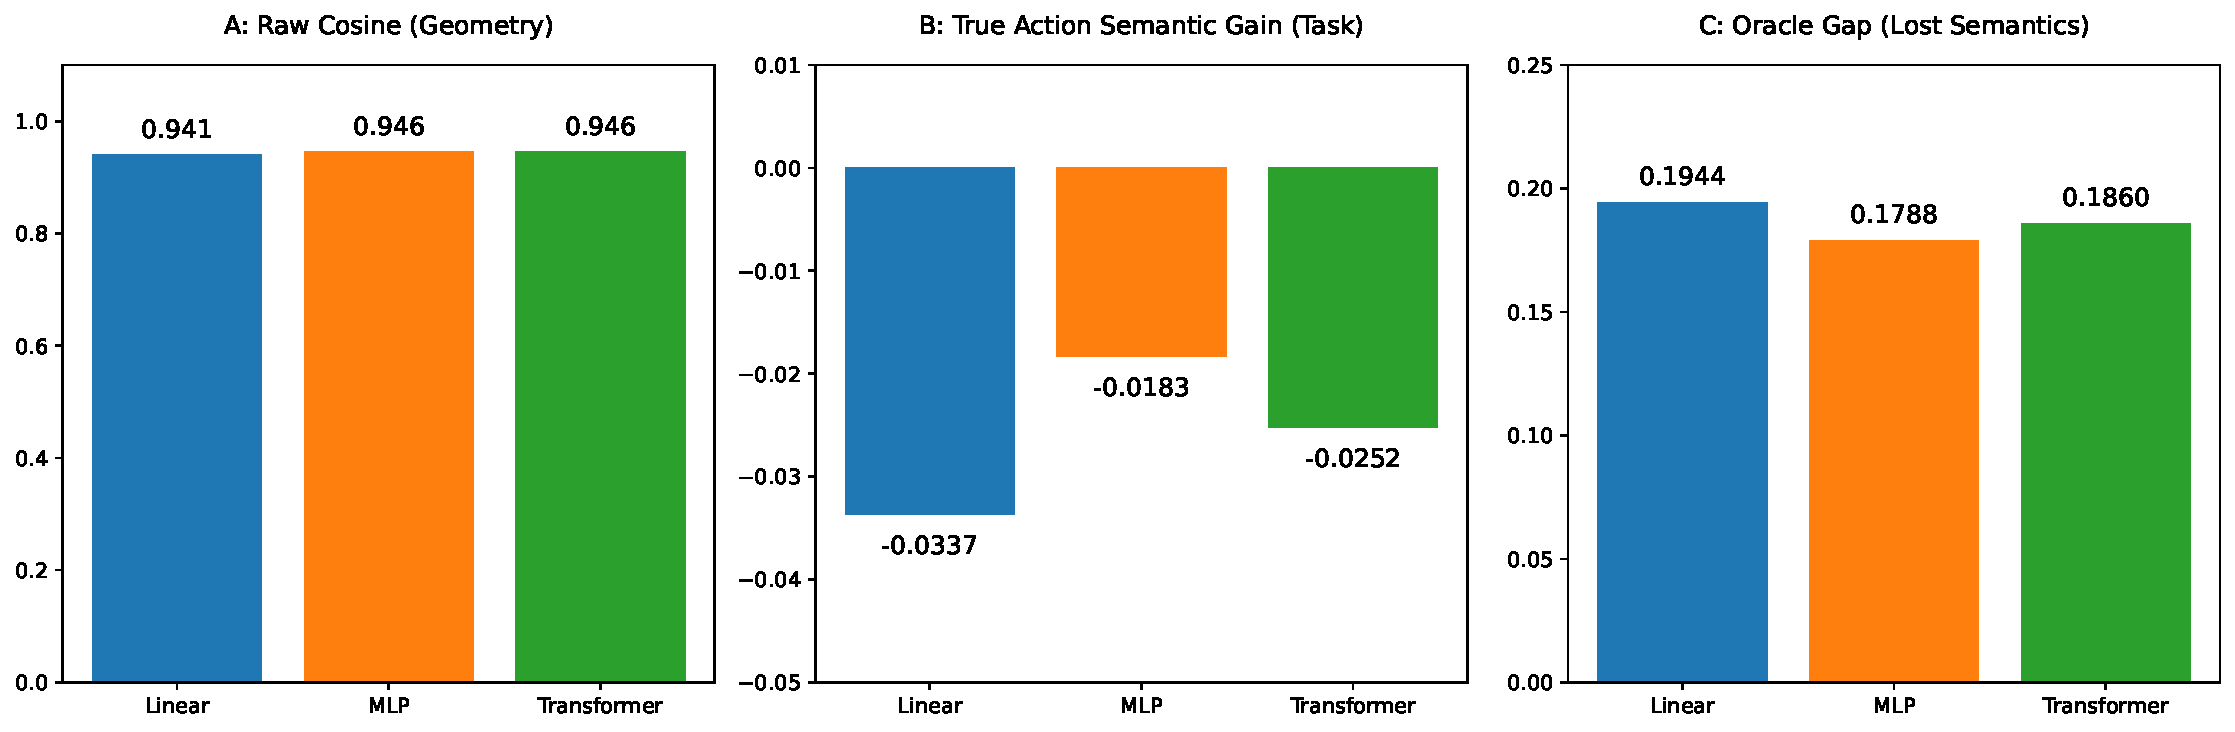
\includegraphics[width=\linewidth]{fig1.pdf}
    \caption{Geometry versus Semantics in Latent Transitions. Panel A displays raw Cosine similarity (Geometry), whereas Panel B and Panel C depict True Action Semantic Gain and Oracle Gap (Semantics). Despite maintaining high geometric similarity ($\approx 0.94$), the evaluated transition architectures do not produce positive True Action Semantic Gain.}
    \label{fig:main_geo_sem}
\end{figure*}

\subsection{Teacher Oracle Ceiling}
The linear probes successfully decode task-critical information from the frozen TinyLlama representations, establishing an empirical reference ceiling for task information decodable by the chosen probe.

\subsection{Architecture-Level Results}
Table \ref{tab:main_results} reports the performance of the three transition architectures across the audited Phase 3 study. The metrics demonstrate a consistently non-zero Oracle Gap across all evaluated models.

\begin{table}[H]
\centering
\caption{Primary Results (Mean $\pm$ 95\% CI Half-Width)}
\label{tab:main_results}
\begin{tabular}{lrr}
\toprule
Architecture & Oracle Gap & True Action SG \\
\midrule
Linear & $0.1944 \pm 0.0659$ & $-0.0337 \pm 0.0645$ \\
MLP & $0.1788 \pm 0.0154$ & $-0.0183 \pm 0.0165$ \\
Transformer & $0.1860 \pm 0.0135$ & $-0.0252 \pm 0.0127$ \\
\bottomrule
\end{tabular}
\end{table}

\subsection{Geometry--Semantics Mismatch}
A central finding is the stark divergence between geometric reconstruction and semantic fidelity (visualized conceptually in Figure \ref{fig:main_geo_sem}). Despite high geometric similarity to the correct target vector (approximately $0.941-0.947$), all nine audited runs produced negative True Action Semantic Gain. This is consistent with a representation that remains close to the teacher target geometrically while failing to recover the task-relevant information captured by the chosen probes. The Mean-Centered Cosine values, roughly $0.30-0.32$, further underscore that standard cosine similarity inflates performance due to the latent space's spatial inertia.

\subsection{Action-Control Ablations}
The results provide limited evidence that the tested transitions consistently derive semantic benefit from the supplied action. The True Action condition performs comparably to the Shuffled and Constant control settings, with negative SG in almost all evaluations.

\subsection{Statistical Analysis}
We formally tested whether the architecture choice systematically affects the Oracle Gap. The comprehensive statistical tests are reported in Table \ref{tab:stats}. A Welch's ANOVA yields $F(2,3.59)=1.1748$ with $p=0.4050$, which did not provide statistically significant evidence of differences in mean Oracle Gap across architectures. Holm-adjusted pairwise Welch $t$-tests likewise show no statistically significant differences. To verify whether initialization variance masked architecture effects, we additionally conducted a paired sensitivity analysis blocking by random seed; this approach also yielded no statistically significant architecture-level differences. Although large effect sizes were observed (e.g., Cohen's $d = -1.221$ for MLP vs Transformer), these effect-size estimates are exploratory and should be interpreted cautiously given the very small number of independent seeds. The study does not provide statistically significant evidence of architecture-level differences, and the low seed count ($n=3$) makes the result inconclusive regarding architectural equivalence.

\begin{table}[H]
\centering
\caption{Statistical Tests (Welch ANOVA and Pairwise t-tests)}
\label{tab:stats}
\begin{tabular}{lrrrr}
\toprule
Comparison / Test & Statistic & $p$ & Corrected $p$ & Effect \\
\midrule
Welch ANOVA & $F=1.1748$ & $0.4050$ & --- & --- \\
MLP vs Transformer & $-1.495$ & $0.2104$ & $0.6311$ & $d=-1.221$ \\
Linear vs MLP & $0.987$ & $0.4188$ & $0.8375$ & $d=0.806$ \\
Linear vs Transformer & $0.537$ & $0.6413$ & $0.8375$ & $d=0.438$ \\
\bottomrule
\end{tabular}
\end{table}

\subsection{Follow-Up Validation with Larger Teachers}

To assess whether the observed geometry--semantics mismatch was confined to the TinyLlama setting, we conducted follow-up experiments with three additional 7B-parameter teachers: Qwen 2.5, Mistral 7B, and DeepSeek-R1-Distill-Qwen-7B. These experiments were new training runs conducted after the primary Phase 3 study as a follow-up validation stage. They used an MLP transition and were not repeated across the three-seed, three-architecture Phase 3 protocol. Nevertheless, all three Countdown runs exhibited high cosine similarity ($>0.95$) alongside substantial corresponding Oracle Gaps and little or negative semantic advancement relative to the identity baseline. These results provide preliminary evidence that the observed geometry--semantics mismatch is not confined to the TinyLlama setting.

\begin{table}[H]
\centering
\caption{Exploratory Validation with 7B Teachers (Depth 1)}
\label{tab:larger_teachers}
\begin{tabular}{llrrr}
\toprule
Teacher & Domain & Cosine & Oracle Gap\textsuperscript{*} & Semantic Gain\textsuperscript{*} \\
\midrule
Qwen 2.5 7B & Countdown & 0.959 & 0.221 & -0.028 \\
Mistral 7B & Countdown & 0.958 & 0.441 & -0.232 \\
DeepSeek-R1-Distill-Qwen-7B & Countdown & 0.987 & 0.182 & +0.004 \\
Qwen 2.5 7B & Game24 & 0.991 & 0.132 & +0.001 \\
\bottomrule
\multicolumn{5}{p{0.95\columnwidth}}{\small \textsuperscript{*}Exploratory quantities derived from the earlier evaluation pipeline; not included in the primary Phase 3 statistical analysis.}
\end{tabular}
\end{table}

\subsection{Cross-Domain Exploratory Validation}

As a separate cross-domain pilot, we evaluated Qwen 2.5 7B on Game24. The transition achieved cosine similarity of 0.991, while the corresponding semantic gain relative to the identity baseline was approximately +0.001 and the corresponding Oracle Gap was 0.132. This result is consistent with the geometry--semantics mismatch observed on Countdown, although the single-run design and differing protocol prevent statistical generalization.

\section{Discussion}

\subsection{Why Geometry Can Mislead}
High-dimensional LLM representations contain structural scaffolding that does not pertain to the local reasoning step. Minimizing MSE or maximizing cosine similarity encourages the transition model to copy this high-magnitude background information. The resulting state is geometrically close, yet deficient in the sensitive subspace where the actual deductive operation is encoded.

\subsection{Latent Representation Inertia}
The combination of high raw cosine similarity and limited semantic advancement is consistent with an identity-like or inertia-dominated transition behavior. Transitions preserve enough geometry to score $>0.94$ raw cosine similarity, but remain consistent with limited semantic advancement from the initial state.

\subsection{Architecture Capacity}
The data suggests that simply increasing transition-model capacity from Linear to MLP to Transformer does not automatically resolve the semantic advancement problem. All nine audited runs produced negative True Action Semantic Gain and consistently non-zero Oracle Gaps.

\subsection{Representational Smoothing Hypothesis}
We hypothesize a phenomenon we term \textit{representational smoothing}. The transition model may suppress high-variance, task-irrelevant components of the teacher representation, acting as a low-pass filter. While this might occasionally produce representations that are temporarily more linearly decodable by weak probes, it does not reliably preserve correct semantic trajectories. We explicitly bound this as a hypothesis requiring further mechanistic analysis.

\subsection{Implications for Latent Planning Evaluation}
The empirical mismatch demonstrates that latent planning models must be evaluated against semantic references (like the Oracle Gap). Relying on representation-level objective functions risks selecting models that are transitions dominated by representation-space inertia rather than capable deductive reasoners.

\begin{table}[H]
\centering
\caption{Summary of Claims and Evidence}
\label{tab:claims}
\begin{tabular}{p{4.2cm}ll}
\toprule
\textbf{Claim} & \textbf{Evidence} & \textbf{Status} \\
\midrule
Geometric similarity can remain high while semantic gain is negative & 9-run results & Empirical \\
\midrule
Architecture differences are statistically distinguishable & Welch ANOVA & \textbf{Not supported} \\
\midrule
Representational smoothing explains the observations & Probe behavior & Hypothesis \\
\midrule
Results generalize across LLMs/tasks & Not tested & Future work \\
\bottomrule
\end{tabular}
\end{table}

\section{Threats to Validity and Limitations}
Our evaluation is explicitly bounded:
\begin{itemize}
    \item \textbf{Small Seed Count:} With $n=3$, inferential statistical power is extremely low.
    \item \textbf{Single Teacher:} The primary statistical study is conducted with a frozen 1.1B TinyLlama teacher. Follow-up experiments with Qwen 2.5 7B, Mistral 7B, and DeepSeek-R1-Distill-Qwen-7B exhibited qualitatively similar geometry--semantics discrepancies under an earlier MLP-based evaluation protocol. These results provide preliminary cross-teacher evidence, but do not establish a quantitative scaling law. A controlled teacher-scale study beyond 7B remains an important direction for future work.
    \item \textbf{Single Reasoning Domain:} The study isolates the deductive Countdown task.
    \item \textbf{Probe Dependence:} Semantic evaluation inherently depends on the structure of the chosen linear probes.
    \item \textbf{Transition Objective Dependence:} All evaluated transitions were trained using a geometric MSE objective; the study does not establish whether semantic-aware training objectives would behave differently.
\end{itemize}

\section{Broader Impact}
Latent reasoning has the potential to reduce inference cost by avoiding some token-level generation, though this paper does not directly measure or benchmark those savings. Uninterpretable latent transitions risk producing opaque, unaligned reasoning pathways. By emphasizing rigorous semantic validation before deployment, this work aims to contribute to safer, more transparent model-based planning.

\section{Future Work}
Future work must investigate whether representational smoothing genuinely reorganizes semantic manifolds and whether semantically regularized training objectives (rather than purely geometric ones) can close the Oracle Gap for latent transition models.

\section{Conclusion}
We introduced a decoupled evaluation framework for assessing semantic fidelity in latent transition models. Across Countdown experiments with a frozen TinyLlama teacher, Linear, MLP, and Transformer transitions all exhibited substantial Oracle Gaps and generally negative Semantic Gain despite high geometric similarity. Architecture-level differences were not statistically distinguishable under the three-seed design, and the limited sample size prevents claims of equivalence. These findings demonstrate that geometric reconstruction metrics alone are insufficient evidence of semantic state preservation in the evaluated latent-transition setting.

\section*{Appendix: Phase 3 Raw Results}
Table \ref{tab:raw_results_app} presents the complete set of raw metrics obtained across all nine audited experimental runs in Phase 3. 
\begin{table}[H]
\centering
\caption{Complete Phase 3 Run-Level Metrics}
\label{tab:raw_results_app}
\begin{tabular}{lrrrrr}
\toprule
Arch. & Seed & True SG & Oracle SG & Oracle Gap & Cosine \\
\midrule
Linear & 42 & -0.0195 & 0.1603 & 0.1798 & 0.941 \\
Linear & 43 & -0.0640 & 0.1610 & 0.2250 & 0.941 \\
Linear & 44 & -0.0177 & 0.1605 & 0.1783 & 0.940 \\
MLP & 42 & -0.0255 & 0.1605 & 0.1860 & 0.946 \\
MLP & 43 & -0.0149 & 0.1605 & 0.1755 & 0.946 \\
MLP & 44 & -0.0144 & 0.1605 & 0.1750 & 0.945 \\
Trans. & 42 & -0.0206 & 0.1608 & 0.1814 & 0.945 \\
Trans. & 43 & -0.0237 & 0.1608 & 0.1845 & 0.946 \\
Trans. & 44 & -0.0314 & 0.1605 & 0.1920 & 0.947 \\
\bottomrule
\end{tabular}
\end{table}

\begin{thebibliography}{00}
\bibitem{hafner2020dream} D. Hafner, T. Lillicrap, J. Ba, and M. Norouzi, ``Dream to control: Learning behaviors by latent imagination,'' in \textit{ICLR}, 2020.
\bibitem{schrittwieser2020mastering} J. Schrittwieser et al., ``Mastering atari, go, chess and shogi by planning with a learned model,'' \textit{Nature}, vol. 588, no. 7839, pp. 604--609, 2020.
\bibitem{belrose2023eliciting} N. Belrose, Z. Furman, L. Logan, C. Pehlevan, and J. Steinhardt, ``Eliciting latent predictions from transformers with the tuned lens,'' \textit{arXiv:2303.08112}, 2023.
\bibitem{alain2017understanding} G. Alain and Y. Bengio, ``Understanding intermediate layers using linear classifier probes,'' in \textit{ICLR}, 2017.
\bibitem{lecun2022path} Y. LeCun, ``A path towards autonomous machine intelligence,'' \textit{Open Review}, vol. 62, 2022.
\bibitem{assran2023self} M. Assran et al., ``Self-supervised learning from images with a joint-embedding predictive architecture,'' in \textit{CVPR}, 2023, pp. 15619--15629.
\bibitem{bardes2024vjepa} A. Bardes et al., ``V-jepa: Latent video prediction for visual representation learning,'' \textit{arXiv:2404.08471}, 2024.
\end{thebibliography}

\end{document}
